
\chapter{Description du jeu de données}

Dans cette partie nous détaillerons l'étude réalisée sur le jeu de données.
Cette étude permet notamment de faire ressortir les corrélations entre les variables
et de mettre en avant les variables les plus déterminantes dans la prédiction du type de 
réclamation. De plus c'est à cette occasion que la réflexion sur la transformation des variables
existantes ou la création de nouveaux features va émerger.

\section{Résumé statistique et première observations}

Le jeu de données de test est composée de 99 995 observations.
Le jeu de données d'entraînement est composé de 100 000 observations dont les fréquences 
de chacun des types de réclamations sont les suivantes :

\begin{itemize}
\item '-' : 50\% 
\item 'NOT_RECEIVED' : 14,8\%
\item 'SELLER_CANCEL_POSTERIORI' : 13,8\%
\item 'WITHDRAWAL' : 7\%
\item ‘DAMAGED' : 5,9\%
\item 'DIFFERENT' : 4,3\%
\item 'UNDEFINED' : 4,1\%
\item 'FAKE' : 0,2\%
\end{itemize}

On note qu'il y a donc 50\% de réclamations et 50\% de non réclamation sur les données 
d'entraînement. De plus, les fréquences des types de réclamations ne sont pas équilibrées,
avec notamment une fréquence très basse pour la déclaration de faux (0,2\%). Pour comparer
nos modèles nous utiliserons donc une métrique de type AUC, plus adaptée à ce type de 
problème. 

La plupart des variables sont catégorielles :

\begin{itemize}
\item Variables nominales : 
	\begin{itemize}
	\item SHIPPING_MODE (11 niveaux)
	\item BUYER_DEPARTMENT (100 niveaux)
	\item BUYING_DATE (10 niveaux)
	\item SELLER_COUNTRY (39 niveaux)
	\item SELLER_DEPARTMENT (98 niveaux)
	\item PRODUCT_TYPE (137 niveaux)
	\item PRODUCT_FAMILY (12 niveaux)
	\end{itemize}
\item Variables dichotomiques/binaires :
	\begin{itemize}
	\item WARRANTIES_FLG
	\item CARD_PAYMENT
	\item COUPON_PAYMENT
	\item RSP_PAYMENT
	\item WALLET_PAYMENT
	\end{itemize}
\item Variables ordinales :
	\begin{itemize}
	\item SHIPPING_PRICE (5 niveaux)
	\item WARRANTIES_PRICE (5 niveaux)
	\item PRICECLUB_STATUS (5 niveaux)
	\item PURCHASE_COUNT (6 niveaux)
	\item SELLER_SCORE_COUNT (5 niveaux)
	\item ITEM_PRICE (8 niveaux)
	\end{itemize}
\item Variables quantitatives :
	\begin{itemize}
	\item REGISTRATION_DATE (17 valeurs distinctes)
	\item BUYER_BIRTHDAY_DATE (107 valeurs distinctes)
	\item SELLER_SCORE_AVERAGE (31 valeurs distinctes)
	\end{itemize}
\end{itemize}

Les variables quantitatives pourront ici être transformées en variables catégorielles.
La date de naissance de l'acheteur pourra par exemple être convertie en catégories d'âge.    
    
Nous pouvons de plus noter que certaines variables ont beaucoup de valeurs manquantes, il 
faudra donc réfléchir à la méthode employée pour combler ces valeurs manquantes :

\begin{itemize}
\item WARRANTIES_PRICE : 96603 / 96.6\% de valeurs manquantes
\item SHIPPING_PRICE : 67610 / 67.6\% de valeurs manquantes
\item BUYER_BIRTHDAY_DATE : 5836 / 5.8\% de valeurs manquantes
\end{itemize}

Aussi, nous notons que les variables binaires ne sont pas équilibrées :

\begin{itemize}
\item WARRANTIES_FLG : 96603 / 96.6\% de 0
\item COUPON_PAYMENT : 94271 / 94.3\% de 0
\item CARD_PAYMENT : 10407 / 89,6\% de 1
\end{itemize}

Certaines variables catégorielles ont beaucoup de niveaux, il faudra donc envisager 
l'éventualité de les modifier avant de les transformer en tableaux d'indicatrices, ce qui
augmenterait considérablement le nombre de variables :

\begin{itemize}
\item PRODUCT_TYPE : 137 valeurs distinctes
\item BUYER_DEPARTMENT 100 valeurs distinctes
\item SELLER_DEPARTMENT 98 valeurs distinctes
\end{itemize}

Nous remarquons de plus que le jeu de données possède 3238 lignes dupliquées. Les
données ont été rendues anonymes, on ne peut donc pas identifier les acheteurs ou les
vendeurs mais il est cependant envisageable que certains individus apparaissent dans 
plusieurs transactions similaires.

\section{Description exhaustive des variables}

\textbf{SHIPPING_MODE et SHIPPING_PRICE :}

Les moyens de livraisons peu populaires ont en moyenne plus de réclamations que les autres.
Pour exemple le moyen de livraison PICKUP avec 73,3\% de réclamations bien plus élevé que 
les 50\% de moyenne.

MONDIAL_RELAY_PREPAYE (46\%), SUIVI (46\%) and NORMAL (47\%) sont les moyens de livraison
les plus fiables.

La livraison NORMAL a le taux le plus élevé de réclamations NOT_RECEIVED (16\%) mais a les taux
de WITHDRAWAL (4\%) et de UNDEFINED (2\%) les plus bas

CHRONOPOST a le plus haut taux de réclamations DAMAGED.

Paradoxalement, le taux de réclamations évolue positivement avec le coût de la livraison.
En particulier les réclamations UNDEFINED et WITHDRAWAL sont plus probables lorsque
le prix du transport est élevé. 

\begin{center}
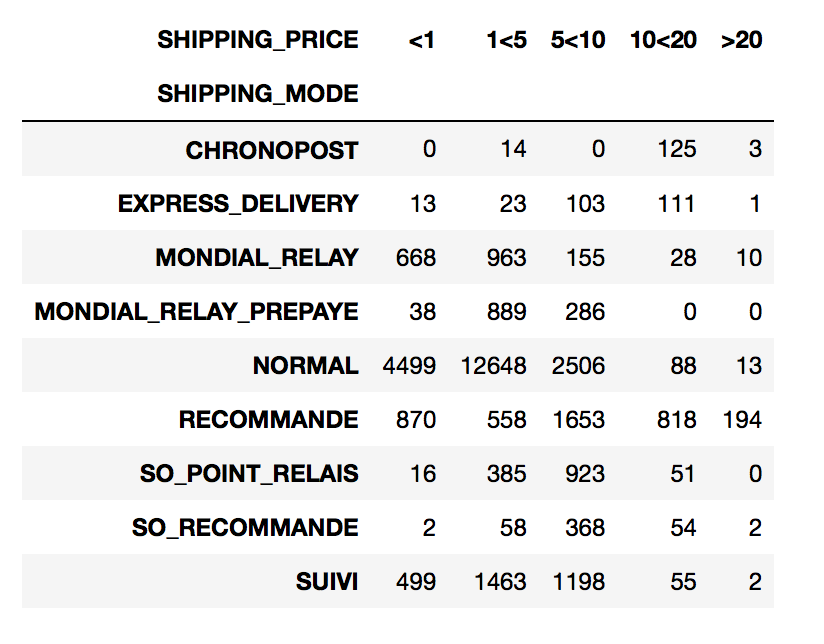
\includegraphics[scale=0.5]{assets/shipping} 
\end{center}

De plus, il y a une corrélation claire entre SHIPPING_MODE et SHIPPING_PRICE. Par exemple,
un SHIPPING_PRICE de plus de 20 a de grandes chances d'être de type RECOMMANDE.

\textbf{WARRANTIES_FLG et WARRANTIES_PRICE :}

Les personnes possédant une garantie sont plus susceptibles de porter des réclamations, en 
particulier de type WITHDRAWAL. Ceci est logique étant donné que le retrait peu être 
facilité par la prise d'une garantie.

Nous n'observons pas de corrélation claires entre le prix de la garantie et le type de
réclamation.

\textbf{PRICECLUB_STATUS :}

Cette variable est liée au nombre de points accumulés en effectuant des actions telles que
vendre des produits, parrainer un ami ou encore utiliser l'application PrimeMinister.
Avec ces points l'utilisateur peut occasionnellement bénéficier d'offres et de réductions.

Il n'y a pas de lien clair entre PRICECLUB_STATUS et les réclamations.

\textbf{REGISTRATION_DATE et PURCHASE_COUNT :}

\begin{center}
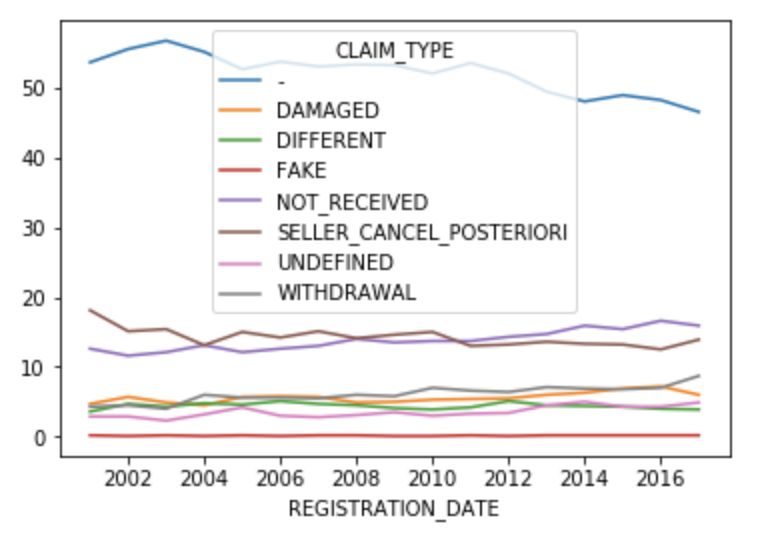
\includegraphics[scale=0.5]{assets/registrationdate} 
\end{center}

Nous observons que les récents utilisateurs ont plus tendance à porter de réclamations.
Il est notable que les acheteurs avec de l'expérience sur le site sont moins susceptibles
de porter des réclamations WITHDRAWAL et UNDEFINED. Cela fait sens car un utilisateur 
habitué a moins de chance de s'être trompé dans sa commande et de la retirer.
Cependant ces acheteurs ont aussi moins tendance à ne pas recevoir leur colis ou à recevoir  
un colis endommagé. Ceci peut s'expliquer par les habitudes des consommateurs qui avec le 
temps n'achètent qu'auprès des vendeurs en qui ils ont confiance.

De manière prévisible, il y a une corrélation importante entre l'année d'inscription de
l'utilisateur et le nombre de commandes passées.

De plus, nous pouvons observer un fossé clair entre les utilisateurs très récents (<5 items 
achetés) et les autres. Pour cette raison il peut être intéressant de créer une variable
supplémentaire pour mettre en avant le fait qu'un utilisateur soit novice ou non.

\textbf{BUYER_BIRTHDAY_DATE :}

\begin{center}
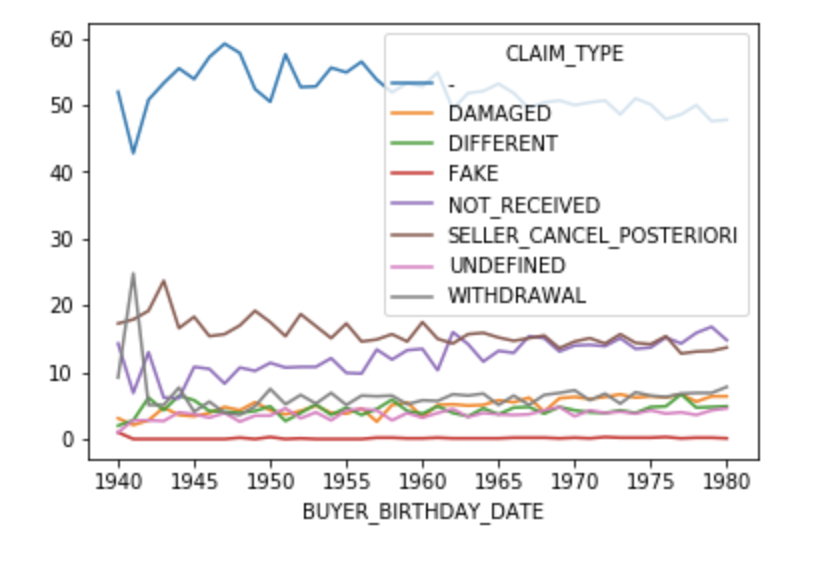
\includegraphics[scale=0.5]{assets/age} 
\end{center}

Une corrélation peu évidente peut être observée entre l'âge et les réclamations. 
En effet, les individus plus jeunes ont une probabilité légèrement plus grande que la moyenne
de porter une réclamation de type NOT_RECEIVED.

\textbf{BUYER_DEPARTMENT, SELLER_DEPARTMENT et SELLER_COUNTRY:}

Pour observer plus facilement l'influence de la localisation des acheteurs et vendeurs
nous avons créé une variable supplémentaire permettant d'identifier les utilisateurs par leur
région au lieu de leur département. 

Il n'y a cependant pas d'influence visible entre la région de l'acheteur et le type de
réclamation si l'acheteur vit en France. Nous pouvons seulement noter qu'en Ile de France
et dans la région PACA les colis sont légèrement plus susceptibles de ne pas arriver
à destination.

Bien entendu, nous pouvons observer que les colis venant de l'étranger sont plus sujets à 
réclamation. Il peut donc être intéressant de créer une variable binaire supplémentaire 
pour mettre l'accent sur le fait que le colis vienne de l'étranger ou non.

On peut noter cependant que certains pays européens ont des taux de réclamations 
proches de la moyenne voir meilleurs (GERMANY : 39,1\%, BELGIUM : 41,8\%, LUXEMBOURG : 41,5\%),
alors que les colis provenant d'autres pays européens proches ont un taux de réclamations pour colis 
non reçu beaucoup plus élevé que la moyenne (19,2\% pour UNITED KINGDOM). 
Il semble donc difficile de regrouper ces pays en catégories et il sera nécessaire de créer
une indicatrice pour chacun de ces pays lors de la phase de feature engineering.

\textbf{BUYING_DATE :}

Cette variable est codé au format 'MM/AAAA' dont nous extrayons uniquement le mois qui est ici 
l'élément qui nous intéresse car toutes les ventes sont réalisées sur l'année 2017.

Nous remarquons d'ailleurs que les données s'arrêtent au mois d'octobre, ce qui est regrettable
puisque la période de Noël, particulièrement prolifique pour les sites de e-commerce, n'est 
pas représentée. Il aurait été intéressant de visualiser l'impact de cette période sur les
réclamations.

Dans ce jeu de données, le mois de Janvier est celui où le plus de commandes sont réalisées,
et c'est aussi le mois où le plus de réclamations sont faites. De même, le mois d'Octobre
est le plus calme en terme de ventes mais aussi en terme de pourcentage de réclamations
faites. La tendance est donc que plus il y a de flux de commandes plus il risque d'y avoir
des réclamations.

\textbf{SELLER_SCORE_COUNT et SELLER_SCORE_AVERAGE :}

Logiquement, nous observons que le nombre de produits vendus par le vendeur est négativement
corrélé avec le taux de réclamations portées. De même, les vendeurs avec les meilleurs
notes moyennes sont les plus fiables. En particulier, les vendeurs avec une note moyenne de
49/50 sont peu nombreux (3994) et au dessus du lot en terme de fiabilité (seulement 12,4\%
de réclamations). Il peut donc être interessant de leur attribuer une variable binaire pour 
renforcer cet écart de fiabilité.

\begin{center}
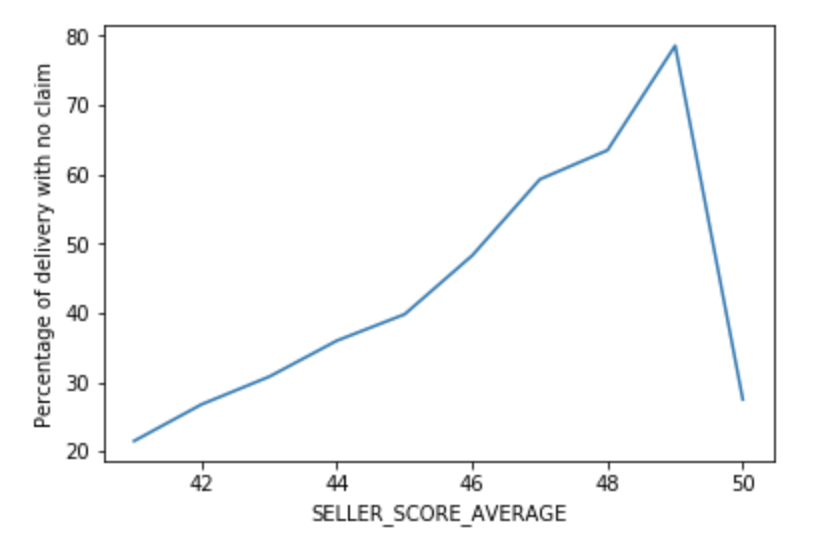
\includegraphics[scale=0.5]{assets/sellerscore} 
\end{center}

Cependant, il faut noter qu'un très petit nombre de vendeurs (51) ont une note moyenne 
maximale de 50/50 et ont cependant un taux de réclamations moyen très élevé (72,5\%) comme
on peut le voir ci-dessus.
Ces vendeurs sont peut-être des comptes fake qui ont réussis à obtenir la note maximale
pour attirer des clients, ou bien des anomalies. Dans tous les cas, il ne faut pas les 
classer parmi les bons vendeurs. Il ne faut pas non plus les considérer comme des outliers
et les retirer du jeu de données car le taux de réclamations qui est lié à ces vendeurs est 
significatif et peut contribuer à améliorer notre prédicteur.

Nous observons de plus une corrélation importante et prévisible entre SELLER_SCORE_COUNT et 
SELLER_SCORE_AVERAGE.

\textbf{PRODUCT_TYPE et PRODUCT_FAMILY :}

Nous remarquons que les produits appartenant à la famille ELECTRONICS ont le taux le plus 
élevé de réclamations DAMAGED (10,8\% contre 5,1\% en moyenne). En effet les produits
électroniques tels qu'une télévision sont plus fragiles et susceptibles d'être 
endommagé lors du transport.


\textbf{ITEM_PRICE :}

Les produits les moins chers sont moins susceptibles de mener à une réclamation.
En particulier les réclamations pour FAKE sont quasiment toujours des produits peu chers.
De même ce sont surtout les achats peu chers qui risquent de ne pas arriver à destination.
Les produits coûteux ont en revanche plus de chance de mener à un retrait de commande.

Les produits dont le prix est compris dans l'intervalle 100<500 ont typiquement plus de
chance d'arriver endommagé. Cela correspond au prix des appareils électroniques qui, comme
nous l'avons observé précédemment, sont plus souvent endommagés lors du transport.



























